% Aberdeen style guide should be followed when using this
% layout. Their template powerpoint slide is used to extract the
% Aberdeen color and logo but is otherwise ignored (it has little or
% no formatting in it anyway).
%
% http://www.abdn.ac.uk/documents/style-guide.pdf

%%%%%%%%%%%%%%%%%%%% Document Class Settings %%%%%%%%%%%%%%%%%%%%%%%%%
% Pick if you want slides, or draft slides (no animations)
%%%%%%%%%%%%%%%%%%%%%%%%%%%%%%%%%%%%%%%%%%%%%%%%%%%%%%%%%%%%%%%%%%%%%%
%Normal document mode%
%\documentclass[10pt,compress,unknownkeysallowed]{beamer}
%Draft or handout mode
\documentclass[10pt,compress,handout,ignorenonframetext,unknownkeysallowed]{beamer}


%%%%%%%%%%%%%%%%%%%% General Document settings %%%%%%%%%%%%%%%%%%%%%%%
% These settings must be set for each presentation
%%%%%%%%%%%%%%%%%%%%%%%%%%%%%%%%%%%%%%%%%%%%%%%%%%%%%%%%%%%%%%%%%%%%%%
\newcommand{\shortname}{jefferson.gomes@abdn.ac.uk}
\newcommand{\fullname}{Dr Jeff Gomes}
\institute{School of Engineering}
\newcommand{\emailaddress}{}%jefferson.gomes@abdn.ac.uk}
\newcommand{\logoimage}{../FigBanner/UoAHorizBanner}
\title{Heat, Mass and Momentum Transfer (EX3030/EM40JN)}
\subtitle{Design of Heat Exchangers}
%\subtitle{Module 1.1: Review of Thermodynamics}
\date[ ]{ }



%%%%%%%%%%%%%%%%%%%%%%%%%%%%%%%%%%%%%%%%%%%%%%%%%%%%%%%%%%%%%%%%%%%%%%%%%%%%%%%
% BABEL and LANGUAGES %%%%%%%%%%%%%%%%%%%%%%%%%%%%%%%%%%%%%%%%%%%%%%%%%%%%%%%%%
%%%%%%%%%%%%%%%%%%%%%%%%%%%%%%%%%%%%%%%%%%%%%%%%%%%%%%%%%%%%%%%%%%%%%%%%%%%%%%%
% \usepackage{listings}                   % it is a source code printer for LATEX
                                          % \lstset{language=Python}
                                          % \lstinputlisting{source.py}   % command used to pretty-print stand alone files
\usepackage[english]{babel}               % [french, frenchb, english, ]
    % http://forum.mathematex.net/latex-f6/les-puces-avec-babel-t4256.html
    % http://www.grappa.univ-lille3.fr/FAQ-LaTeX/11.1.html


%%%%%%%%%%%%%%%%%%%%%%%%%%%%%%%%%%%%%%%%%%%%%%%%%%%%%%%%%%%%%%%%%%%%%%%%%%%%%%%
% FONTS and ENCODING %%%%%%%%%%%%%%%%%%%%%%%%%%%%%%%%%%%%%%%%%%%%%%%%%%%%%%%%%%
%%%%%%%%%%%%%%%%%%%%%%%%%%%%%%%%%%%%%%%%%%%%%%%%%%%%%%%%%%%%%%%%%%%%%%%%%%%%%%%
%
% See:
% http://tex.stackexchange.com/questions/59702/suggest-a-nice-font-family-for-my-basic-latex-template-text-and-math-i-am
%

\usepackage{lmodern}        % Latin Modern family of fonts. Very much like Computer Modern, but with many more glyphs 
                            % (e.g., for characters with accents, glyphs, cedillas, etc)
\usepackage[T1]{fontenc}    % fontenc is oriented to output, that is, what fonts to use for printing characters. 
                            % http://tex.stackexchange.com/questions/44694/fontenc-vs-inputenc 
                            % http://tex.stackexchange.com/questions/664/why-should-i-use-usepackaget1fontenc

% Change some fonts or the whole font family (i.e. serif, sans serif, monospace, and 'math')
    % \usepackage[varg, cmintegrals, cmbraces, ]{newtxtext,newtxmath}  % Other options: libertine, uprightGreek (U.S.) or slantedGreek (ISO), etc...
     \usepackage{tgtermes}                                            % Only serif ("TeX-Gyre" text)
    % \usepackage{kpfonts}                                             % "Kepler" fonts
    % \usepackage{mathpazo}                                            % Based on Hermann Zapf's Palatino font
    % \usepackage{txfonts}                                             % More than a decade old
    % \usepackage{pslatex}                                             % Obsolete?
    %  - \usepackage{mathptmx}
    %  - \usepackage[scaled=.90]{helvet}
    %  - \usepackage{courier}

% \usepackage{textcomp}     % required for special glyphs
% \usepackage{bm}           % load after all math to give access to bold math
\usepackage[utf8]{inputenc} % inputenc allows the user to input accented characters directly from the keyboard; 
                            % utf8x : much broader but less compatible ; latin1 : old?
                            % http://tex.stackexchange.com/questions/44694/fontenc-vs-inputenc

% See:
% http://tex.stackexchange.com/questions/59626/nicely-force-66-characters-per-line
%
% pslatex is a very obsolete package and that its descendant mathptmx is rather inadequate for serious typesetting involving math.
% If you don't need mathematics, other choices based on (Linotype) Times Roman are
%  - tgtermes
%  - newtxtext (based on txfonts, but with corrected metrics) (with its companion math package newtxmath)
%
%
% See:
% http://www.latex-community.org/forum/viewtopic.php?f=8&t=6637
%
% (times, helvet, courier)
% pslatex and txfonts produce (almost) same resutls.
% pslatex supposedly obsolete
% txfonts supposedly up-to-date
%
%
% See:
% ftp://ftp.rrzn.uni-hannover.de/pub/mirror/tex-archive/info/l2tabu/english/l2tabuen.pdf
% or 
% ftp://ftp.dante.de/tex-archive/info/l2tabu/english/l2tabuen.pdf
% in
% 2.3.3 pslatex.sty
%
% pslatex uses a Courier font scaled too narrowly.
% Its main disadvantage is that it does not work with T1 and TS1 encodings.
% So replace:
% \usepackage{pslatex} or \usepackage{txfonts}
% by all three:
% - \usepackage{mathptmx}
% - \usepackage[scaled=.90]{helvet}
% - \usepackage{courier}
%
%
% See:
% http://xpt.sourceforge.net/techdocs/language/latex/latex32-LaTeXAndFonts/single/
% or http://thirteen-01.stat.iastate.edu/wiki/LaTeXFonts
% or http://www.tex.ac.uk/tex-archive/info/beginlatex/html/chapter8.html
%
% When changing fonts, you can change all of the default fonts at once with the following commands:
% 
% Command     Changes the defaults to
% 
% times       Times, Helvetica, Courier
% pslatex     same as Times, but uses a specially narrowed Courier. This is preferred over Times because of the way it handles Courier.
% newcent     New Century Schoolbook, Avant Garde, Courier
% palatino    Palatino, Helevetica, Courier
% palatcm     changes the Roman to Palatino only, but uses CM mathematics
% kpfonts     "Kepler" fonts. A very nicely evolved set of fonts also based originally on Palatino, but with many special features.
%
%
% See:
% http://tex.stackexchange.com/questions/59702/suggest-a-nice-font-family-for-my-basic-latex-template-text-and-math-i-am
%
% There are, of course, many other font packages, most of which provide "only" text-mode fonts.
% Among these are the "TeX-Gyre" font families: 
%  - Termes (a Times Roman clone), 
%  - Pagella (a Palatino clone), and 
%  - Schola (a Century Schoolbook clone); 
% one would load the packages tgtermes, tgpagella, and tgschola, respectively, to access these fonts.
% However, as these are text fonts, you still need to choose a suitable math font.
% 
% Still another possibility you may want to look into is the Linux Libertine font family, to be loaded via the libertine-legacy package.
% If you like this text font and wish to employ the newtxmath package, be sure to load the newtxmath package with the libertine option set;
% doing so will set up a special set of math-mode fonts that harmonizes well with the libertine text fonts.
% 
%
% See also:
% http://tex.stackexchange.com/questions/56876/times-new-roman-fonts-and-maths-without-mathptmx
%
%
% For a comparison, in:
% /home/christophe/Personal/Truc_Et_Astuce_Informatik/LaTeX/comparison_font_types/,
% see: 
% computer.pdf  lmodern.pdf  pslatex.pdf  test_font_type.pdf  three_replacements.pdf  txfonts.pdf
%


%%%%%%%%%%%%%%%%%%%%%%%%%%%%%%%%%%%%%%%%%%%%%%%%%%%%%%%%%%%%%%%%%%%%%%%%%%%%%%%
% AMS MATH %%%%%%%%%%%%%%%%%%%%%%%%%%%%%%%%%%%%%%%%%%%%%%%%%%%%%%%%%%%%%%%%%%%%
%%%%%%%%%%%%%%%%%%%%%%%%%%%%%%%%%%%%%%%%%%%%%%%%%%%%%%%%%%%%%%%%%%%%%%%%%%%%%%%
% \usepackage{amsmath}      % loads amstext, amsbsy, amsopn but not amssymb
                            % equation stuff (eqref, subequations, equation, align, gather, flalign, multline, alignat, split...)
% \usepackage{amsfonts}     % may be redundant with amsmath
% \usepackage{amssymb}      % may be redundant with amsmath
% \numberwithin{equation}{section}  % reset equation counters at start of each "section" and prefix numbers by section number
% \numberwithin{figure}{section}    % reset figure   counters at start of each "section" and prefix numbers by section number


%%%%%%%%%%%%%%%%%%%%%%%%%%%%%%%%%%%%%%%%%%%%%%%%%%%%%%%%%%%%%%%%%%%%%%%%%%%%%%%
% LAY OUT %%%%%%%%%%%%%%%%%%%%%%%%%%%%%%%%%%%%%%%%%%%%%%%%%%%%%%%%%%%%%%%%%%%%%
%%%%%%%%%%%%%%%%%%%%%%%%%%%%%%%%%%%%%%%%%%%%%%%%%%%%%%%%%%%%%%%%%%%%%%%%%%%%%%%
%
% See:
% http://tex.stackexchange.com/questions/59626/nicely-force-66-characters-per-line
% (must be after pslatex, tgterms, etc...)
%
% a) (but works mostly for a4paper, and changes top and bottom margin too...)
% \usepackage[DIV=calc]{typearea}
%
% or
%
% b) (but you have to choose the value and the margin ratio depending on the class...)
% \newlength{\alphabet}
% \settowidth{\alphabet}{\normalfont abcdefghijklmnopqrstuvwxyz}
% \usepackage{geometry}
% \geometry{%
% textwidth=2.5\alphabet,% (Note: 2.5 * 26 = 65)
% hmarginratio={2:3}}    % (Problem: geometry uses 2:3 as default for twoside and 1:1 for oneside,
%                        % independently of what the class thinks about the margins)

% \usepackage{layout}       % use \layout in the tex file to see the values
% \usepackage{layouts}      % it extends the functionality of layout, allowing you to do much, much more
                            % some commands: \pagelayout, \pagevalues, \pagedesign, ...
% \usepackage[cm]{fullpage} % set 'default' full page
% \usepackage{geometry}     % very customizable margins. Under some (rare) circumstances, should be loaded after hyperref
% \usepackage{anysize}      % \marginsize{left}{right}{top}{bottom}
% \usepackage{pdflscape}    % include landscape layout pages (automatically rotate pages in pdf file for easier reading)
% \usepackage{multicol}     % for multi column environment
\usepackage{lipsum}         % to fill in with arbitrary text
\widowpenalty = 4000        % help suppress widows,  default = 4,000 (?), from 0 to 10 000 (from 300 to 1 000 recommended, 10 000 not recommended)
\clubpenalty  = 4000        % help suppress orphans, default = 4,000 (?), from 0 to 10 000 (from 300 to 1 000 recommended, 10 000 not recommended)
\usepackage[final, babel]{microtype} % many good lay-out/justification effects, see:
                                     % texblog.net/latex-archive/layout/pdflatex-microtype/


%%%%%%%%%%%%%%%%%%%%%%%%%%%%%%%%%%%%%%%%%%%%%%%%%%%%%%%%%%%%%%%%%%%%%%%%%%%%%%%
% EMBED FILEs %%%%%%%%%%%%%%%%%%%%%%%%%%%%%%%%%%%%%%%%%%%%%%%%%%%%%%%%%%%%%%%%%
%%%%%%%%%%%%%%%%%%%%%%%%%%%%%%%%%%%%%%%%%%%%%%%%%%%%%%%%%%%%%%%%%%%%%%%%%%%%%%%
\usepackage{embedfile}    % embed (attach) any files (eg tex source) to a PDF document.
                          % Currently only supported driver is pdfTEX >= 1.30 in PDF mode
%\embedfile{to_post.tex}


%%%%%%%%%%%%%%%%%%%%%%%%%%%%%%%%%%%%%%%%%%%%%%%%%%%%%%%%%%%%%%%%%%%%%%%%%%%%%%%
% EASY EDITS %%%%%%%%%%%%%%%%%%%%%%%%%%%%%%%%%%%%%%%%%%%%%%%%%%%%%%%%%%%%%%%%%%
%%%%%%%%%%%%%%%%%%%%%%%%%%%%%%%%%%%%%%%%%%%%%%%%%%%%%%%%%%%%%%%%%%%%%%%%%%%%%%%
\usepackage{ifdraft}        % ask for selective behavior depending on the draft option (used for waterdraftmark, not draftmark)
% \usepackage{comment}      % provide new {comment} environment: all text inside the environment is ignored.
% \usepackage{fixme}        % allow nice comment / warning system, displayed in draft mode in right margin ; % [status=draft]
% \usepackage{lineno}       % number all lines in left margin if activated with \linenumbers
% \linenumbers


%%%%%%%%%%%%%%%%%%%%%%%%%%%%%%%%%%%%%%%%%%%%%%%%%%%%%%%%%%%%%%%%%%%%%%%%%%%%%%%
% GRAPHICX %%%%%%%%%%%%%%%%%%%%%%%%%%%%%%%%%%%%%%%%%%%%%%%%%%%%%%%%%%%%%%%%%%%%
%%%%%%%%%%%%%%%%%%%%%%%%%%%%%%%%%%%%%%%%%%%%%%%%%%%%%%%%%%%%%%%%%%%%%%%%%%%%%%%
% \usepackage[final]{graphicx} % options = [final]  = all graphics displayed, regardless of draft option in class
                               % options = [pdftex] = necessary (?) if import PDF files
                               % no option : when importing ps- and eps-files (?)
% \graphicspath{{../images/}}  % tell LaTeX where to look for images
% \DeclareGraphicsExtensions{.pdf, .PDF, .jpg, .JPG, .jpeg, .JPEG, .png, .PNG, .bmp, .BMP, .eps, .ps}
\usepackage{float}                      % Improved interface for floating objects ; add [H] option


%%%%%%%%%%%%%%%%%%%%%%%%%%%%%%%%%%%%%%%%%%%%%%%%%%%%%%%%%%%%%%%%%%%%%%%%%%%%%%%
% FILIGREE %%%%%%%%%%%%%%%%%%%%%%%%%%%%%%%%%%%%%%%%%%%%%%%%%%%%%%%%%%%%%%%%%%%%
%%%%%%%%%%%%%%%%%%%%%%%%%%%%%%%%%%%%%%%%%%%%%%%%%%%%%%%%%%%%%%%%%%%%%%%%%%%%%%%
% draftmark : newer and better package but not on Phil's computers,
% in particular, draftmark has a "ifdraft" option included...
%
\ifdraft{
\usepackage{draftwatermark} % add watermark ("draft", "confidential"...)
                            % option: [firstpage] (insert on only the first page)
\SetWatermarkText{COPY~---~DRAFT}
\SetWatermarkAngle{55}
\SetWatermarkScale{6.0}
\SetWatermarkLightness{0.85}
\SetWatermarkFontSize{12 pt}
}{}


\renewcommand{\insertframenumber}{\theframenumber}
\renewcommand{\theframenumber}{\thesection-\arabic{framenumber}}
\renewcommand{\thesubsectionslide}{\thesection-\arabic{framenumber}}
\setbeamertemplate{headline}[text line]{This is frame: \insertframenumber}
\AtBeginSection{\setcounter{framenumber}{0}}


%%%%%%%%%%%%%%%%%%%% Template settings %%%%%%%%%%%%%%%%%%%%%%%%%%%%%%%
% You shouldn't have to change below this line, unless you want to.
%%%%%%%%%%%%%%%%%%%%%%%%%%%%%%%%%%%%%%%%%%%%%%%%%%%%%%%%%%%%%%%%%%%%%%
\usecolortheme{whale}
\useoutertheme{infolines}

% Use the fading effect for items that are covered on the current
% slide.
\beamertemplatetransparentcovered

% We abuse the author command to place all of the slide information on
% the title page.
\author[\shortname]{%
  \fullname\\\ttfamily{\emailaddress}
}


%At the start of every section, put a slide indicating the contents of the current section.
\AtBeginSection[] {
  \begin{frame}
    \frametitle{Section Outline}
    \tableofcontents[currentsection]
  \end{frame}
}

% Allow the inclusion of movies into the Presentation! At present,
% only the Okular program is capable of playing the movies *IN* the
% presentation.
\usepackage{multimedia}
\usepackage{animate}

%% Handsout -- comment out the lines below to create handstout with 4 slides in a page with space for comments
\usepackage{handoutWithNotes}

\mode<handout>
{
\usepackage{pgf,pgfpages}

\pgfpagesdeclarelayout{2 on 1 boxed with notes}
{
\edef\pgfpageoptionheight{\the\paperheight} 
\edef\pgfpageoptionwidth{\the\paperwidth}
\edef\pgfpageoptionborder{0pt}
}
{
\setkeys{pgfpagesuselayoutoption}{landscape}
\pgfpagesphysicalpageoptions
    {%
        logical pages=4,%
        physical height=\pgfpageoptionheight,%
        physical width=\pgfpageoptionwidth,%
        last logical shipout=2%
    } 
\pgfpageslogicalpageoptions{1}
    {%
    border code=\pgfsetlinewidth{1pt}\pgfstroke,%
    scale=1,
    center=\pgfpoint{.25\pgfphysicalwidth}{.75\pgfphysicalheight}%
    }%
\pgfpageslogicalpageoptions{2}
    {%
    border code=\pgfsetlinewidth{1pt}\pgfstroke,%
    scale=1,
    center=\pgfpoint{.25\pgfphysicalwidth}{.25\pgfphysicalheight}%
    }%
\pgfpageslogicalpageoptions{3}
    {%
    border shrink=\pgfpageoptionborder,%
    resized width=.7\pgfphysicalwidth,%
    resized height=.5\pgfphysicalheight,%
    center=\pgfpoint{.75\pgfphysicalwidth}{.29\pgfphysicalheight},%
    copy from=3
    }%
\pgfpageslogicalpageoptions{4}
    {%
    border shrink=\pgfpageoptionborder,%
    resized width=.7\pgfphysicalwidth,%
    resized height=.5\pgfphysicalheight,%
    center=\pgfpoint{.75\pgfphysicalwidth}{.79\pgfphysicalheight},%
    copy from=4
    }%

\AtBeginDocument
    {
    \newbox\notesbox
    \setbox\notesbox=\vbox
        {
            \hsize=\paperwidth
            \vskip-1in\hskip-1in\vbox
            {
                \vskip1cm
                Notes\vskip1cm
                        \hrule width\paperwidth\vskip1cm
                    \hrule width\paperwidth\vskip1cm
                        \hrule width\paperwidth\vskip1cm
                    \hrule width\paperwidth\vskip1cm
                        \hrule width\paperwidth\vskip1cm
                    \hrule width\paperwidth\vskip1cm
                    \hrule width\paperwidth\vskip1cm
                    \hrule width\paperwidth\vskip1cm
                        \hrule width\paperwidth
            }
        }
        \pgfpagesshipoutlogicalpage{3}\copy\notesbox
        \pgfpagesshipoutlogicalpage{4}\copy\notesbox
    }
}
}

%\pgfpagesuselayout{2 on 1 boxed with notes}[letterpaper,border shrink=5mm]
%\pgfpagesuselayout{2 on 1 boxed with notes}[letterpaper,border shrink=5mm]


%%%%%%%%%% Chemical Reactions %%%%%%%%%%%%%%%%

\usepackage[T1]{fontenc}
\usepackage[utf8]{inputenc}
\usepackage{lmodern}
\usepackage[version=3]{mhchem}
\makeatletter
\newcounter{reaction}
%%% >> for article <<
%\renewcommand\thereaction{C\,\arabic{reaction}}
%%% << for article <<
%%% >> for report and book >>
%\renewcommand\thereaction{C\,\thechapter.\arabic{reaction}}
%\@addtoreset{reaction}{chapter}
%%% << for report and book <<
\newcommand\reactiontag{\refstepcounter{reaction}\tag{\thereaction}}
\newcommand\reaction@[2][]{\begin{equation}\ce{#2}%
\ifx\@empty#1\@empty\else\label{#1}\fi%
\reactiontag\end{equation}}
\newcommand\reaction@nonumber[1]{\begin{equation*}\ce{#1}%
\end{equation*}}
\newcommand\reaction{\@ifstar{\reaction@nonumber}{\reaction@}}
\makeatother

%%%%%%%%%%%%%%%%%%%%%%%%%%%%%%%%%%%%%%%%%%%%%%


%%%%% Color settings
\usepackage{color}
%% The background color for code listings (i.e. example programs)
\definecolor{lbcolor}{rgb}{0.9,0.9,0.9}%
\definecolor{UoARed}{rgb}{0.64706, 0.0, 0.12941}
\definecolor{UoALight}{rgb}{0.85, 0.85, 0.85}
\definecolor{UoALighter}{rgb}{0.92, 0.92, 0.92}
\setbeamercolor{structure}{fg=UoARed} % General background and higlight color
\setbeamercolor{frametitle}{bg=black} % General color
\setbeamercolor{frametitle right}{bg=black} % General color
\setbeamercolor{block body}{bg=UoALighter} % For blocks
\setbeamercolor{structure}{bg=UoALight} % For blocks
% Rounded boxes for blocks
\setbeamertemplate{blocks}[rounded]

%%%%% Font settings
% Aberdeen requires the use of Arial in slides. We can use the
% Helvetica font as its widely available like so
% \usepackage{helvet}
% \renewcommand{\familydefault}{\sfdefault}
% But beamer already uses a sans font, so we will stick with that.

% The size of the font used for the code listings.
\newcommand{\goodsize}{\fontsize{6}{7}\selectfont}

% Extra math packages, symbols and colors. If you're using Latex you
% must be using it for formatting the math!
\usepackage{amscd,amssymb} \usepackage{amsfonts}
\usepackage[mathscr]{eucal} \usepackage{mathrsfs}
\usepackage{latexsym} \usepackage{amsmath} \usepackage{bm}
\usepackage{amsthm} \usepackage{textcomp} \usepackage{eurosym}
% This package provides \cancel{a} and \cancelto{a}{b} to "cancel"
% expressions in math.
\usepackage{cancel}

\usepackage{comment} 

% Get rid of font warnings as modern LaTaX installations have scalable
% fonts
\usepackage{type1cm} 

%\usepackage{enumitem} % continuous numbering throughout enumerate commands

% For exact placement of images/text on the cover page
\usepackage[absolute]{textpos}
\setlength{\TPHorizModule}{1mm}%sets the textpos unit
\setlength{\TPVertModule}{\TPHorizModule} 

% Source code formatting package
\usepackage{listings}%
\lstset{ backgroundcolor=\color{lbcolor}, tabsize=4,
  numberstyle=\tiny, rulecolor=, language=C++, basicstyle=\goodsize,
  upquote=true, aboveskip={1.5\baselineskip}, columns=fixed,
  showstringspaces=false, extendedchars=true, breaklines=false,
  prebreak = \raisebox{0ex}[0ex][0ex]{\ensuremath{\hookleftarrow}},
  frame=single, showtabs=false, showspaces=false,
  showstringspaces=false, identifierstyle=\ttfamily,
  keywordstyle=\color[rgb]{0,0,1},
  commentstyle=\color[rgb]{0.133,0.545,0.133},
  stringstyle=\color[rgb]{0.627,0.126,0.941}}

% Allows the inclusion of other PDF's into the final PDF. Great for
% attaching tutorial sheets etc.
\usepackage{pdfpages}
\setbeamercolor{background canvas}{bg=}  

% Remove foot note horizontal rules, they occupy too much space on the slide
\renewcommand{\footnoterule}{}

% Force the driver to fix the colors on PDF's which include mixed
% colorspaces and transparency.
\pdfpageattr {/Group << /S /Transparency /I true /CS /DeviceRGB>>}

% Include a graphics, reserve space for it but
% show it on the next frame.
% Parameters:
% #1 Which slide you want it on
% #2 Previous slides
% #3 Options to \includegraphics (optional)
% #4 Name of graphic
\newcommand{\reserveandshow}[4]{%
\phantom{\includegraphics<#2|handout:0>[#3]{#4}}%
\includegraphics<#1>[#3]{#4}%
}

\newcommand{\frc}{\displaystyle\frac}
\newcommand{\red}{\textcolor{red}}
\newcommand{\blue}{\textcolor{blue}}
\newcommand{\green}{\textcolor{green}}
\newcommand{\purple}{\textcolor{purple}}
\newcommand{\eg}{{\it e.g., }}
\newcommand{\ie}{{\it i.e., }}
\newcommand{\wrt}{{\it wrt }}
\newcommand{\Partial}[3][error]{\left(\frc{\partial #1}{\partial #2}\right)_{#3}}
\newcommand{\mfr}[3][error]{#1_{#2}^{\left(#3\right)}} 
\newcommand{\summation}[3][error]{\sum\limits_{#2}^{#3}#1}


\begin{document}

% Title page layout
\begin{frame}
  \titlepage 
  \vfill%
  \begin{center}
    \includegraphics[clip,width=0.8\textwidth]{\logoimage}
  \end{center}
\end{frame}

% Table of contents
%\frame{ \frametitle{Slides Outline}
%  \tableofcontents
%}


%%%%%%%%%%%%%%%%%%%% The Presentation Proper %%%%%%%%%%%%%%%%%%%%%%%%%
% Fill below this line with \begin{frame} commands! It's best to
% always add the fragile option incase you're going to use the
% verbatim environment.
%%%%%%%%%%%%%%%%%%%%%%%%%%%%%%%%%%%%%%%%%%%%%%%%%%%%%%%%%%%%%%%%%%%%%%

%%%
%%% SECTION
%%%
\section{Introduction} 


%%% SUBSECTION
\subsection{Objectives}

%%%
%%% Slide
%%%
\begin{frame}
 \frametitle{Objectives}
    \begin{columns}
       \begin{column}[l]{0.6\linewidth}
         \hspace{-.70cm}\includegraphics[width=1.1\columnwidth,clip]{./Pics/HE_Utube}
       \end{column}
       \begin{column}[l]{0.4\linewidth}
          \begin{enumerate}
              \item<1-> Heat exchangers (HE) are key-elements in any industrial process from power generation, chemical processing, electronics cooling, refrigeration to automotive, food $\&$ drink, bio-medical etc;
          \end{enumerate}
       \end{column}      
    \end{columns}
          \begin{enumerate}\setcounter{enumi}{1}
              \item<2-> In this module, we will focus on fundamental aspects of design and operation of HE.
          \end{enumerate}
\end{frame}


%%%
%%% SUBSECTION
%%%
\subsection{Bibliography} 

%%%
%%% Slide
%%%
\begin{frame}
 \frametitle{Suggested References}
  Literature relevant for this module:
  \begin{enumerate}[{[}1{]}]
    \item F.P. Incropera, D.P. DeWitt, T.L.Bergman, A.S. Lavine, `Introduction to Heat Transfer' (John Willey $\&$ Sons): Chapter 11.
    \item J.P. Holman, `Heat Transfer', 10$^{th}$ Edition (McGraw-Hill): Chapter 10;
    \item Y.A. Cengel, `Heat Transfer: A Practical Approach', 2$^{nd}$ Edition (McGraw-Hill): Chapter 13;
    \item L. Theodore, `Essential Engineering Calculations Series: Heat Transfer Applications for the Practicing Engineer' (John Willey $\&$ Sons): Chapter 14.
  \end{enumerate}
\end{frame}


%%%
%%% SECTION
%%%
\section{Heat Exchangers} 

%%% SUBSECTION
\subsection{Introduction}

%%%
%%% Slide
%%%
\begin{frame}
 \frametitle{Introduction}
    \begin{enumerate}%\scriptsize
        \item<1-> Heat exchangers are devices that permits \underline{efficient} transfer of heat from a hot fluid to a cold fluid without any, or with direct contact of fluids;
        \item<2-> In other words, they are equipment that are used to thermal energy transfer (\ie \blue{enthalpy}) between:
            \begin{enumerate}%\scriptsize
               \item<2-> two or more fluids;
               \item<2-> solid surface and a fluid or;
               \item<2-> solid particulates and a fluid;
            \end{enumerate}
            at different temperature and in thermal contact;
       \item<3-> The heat transfer to the working fluid may occur through
            \begin{enumerate}%\scriptsize
               \item<3-> internal energy sources, \eg electrical heaters and nuclear fuel elements;
               \item<3-> combustion and chemical reaction, \eg boilers, fired-heaters and fluidised-bed exchangers;
               \item<3-> mechanical devices, \eg scraped surface exchangers, agitated vessels and stirred tank reactors.
            \end{enumerate}
   \end{enumerate}
\end{frame}


%%% SUBSECTION
\subsection{Classification}

%%%
%%% Slide
%%%
\begin{frame}
 \frametitle{HE Classification}
    Heat exchangers may be classified by:
      \begin{enumerate}%\scriptsize
          \item<1-> Number of fluids: 2-, 3- or N-fluids;
          \item<2-> Transfer process:
             \begin{enumerate}
                 \item<2-> indirect contact type: direct transfer type (\ie single- and multiphase flow system); storage type and fluidised beds;
                 \item<2-> direct contact type: immiscible fluids; gas-liquid; and liquid-vapour;
             \end{enumerate}
          \item<3-> Heat transfer mechanisms:
             \begin{enumerate}
                 \item<3-> single-phase convection on both sides;  
                 \item<3-> single-phase convection on one side and two-phase onvection on the other side; 
                 \item<3-> two-phase convection on both sides;
                 \item<3-> combined convection and radiative heat transfer.
             \end{enumerate}
   \end{enumerate}
\end{frame}

%%%
%%% Slide
%%%
\begin{frame}
 \frametitle{HE Classification}
      \begin{enumerate}\setcounter{enumi}{3}
          \item<1-> Flow arrangements:
             \begin{enumerate}
                 \item<1-> single-pass: counterflow; parallel flow; cross-flow; split-flow; divided-flow;
                 \item<2-> multi-pass: 
                    \begin{enumerate}
                       \item<2-> extended surface: cross-counter flow; cross-parallel flow; compound flow;
                       \item<2-> shell-and-tube: parallel counter flow (m-shell passes and n-tube passes); split flow; divide flow;
                       \item<2-> plate: fluid 1 $m$ passes and fluid 2 $n$ passes;
                    \end{enumerate}
             \end{enumerate}
          \item<3-> Construction:
              \begin{enumerate}
                 \item<3-> tubular: double pipe; shell-and-tube (cross-flow and parallel-flow to tubes); spiral tube; pipe-coils;
                 \item<3-> plate-type;
                 \item<3-> extended surface: plate-fin; tube-fin;
                 \item<3-> regenerative: rotary; fixed matrix; rotating hoods
              \end{enumerate}
   \end{enumerate}
\end{frame}

%%%
%%% Slide
%%%
\begin{frame}
 \frametitle{HE Classification}
    \begin{columns}
       \begin{column}[l]{0.58\linewidth}
         \includegraphics[width=1.1\columnwidth,clip]{./Pics/HeatExchangers_Examples}
       \end{column}
       \begin{column}[l]{0.42\linewidth}
          \begin{enumerate}\setcounter{enumi}{5}%\scriptsize
              \item<1-> A more general classification that encompass some of the previous characteristics, includes 3 main types of HE:
                \begin{enumerate}
                  \item<1-> \blue{Recuperative}: heat is transferred from one fluid to another through a dividing wall;
                  \item<2-> \blue{Regenerative}: heat from a hot fluid is stored in a thermal storage medium before being transferred to a cold fluid;
                  \item<3-> \blue{Evaporative}: heat from hot fluid is removed by partial evaporation.
                \end{enumerate}
          \end{enumerate}
       \end{column}      
    \end{columns}
          \begin{enumerate}\setcounter{enumi}{6}%\scriptsize
               \item<4-> Our main focus on this module is to study \underline{\blue{Recuperative HE}}.
          \end{enumerate}
\end{frame}


%%% SUBSECTION
\subsection{HE Configurations}

%%%
%%% Slide
%%%
\begin{frame}
  \frametitle{Configurations and HT mechanisms}
    \begin{columns}
       \begin{column}[l]{0.5\linewidth}
         \includegraphics[width=1.3\columnwidth,clip]{./Pics/HeatExchangers_Classification}
       \end{column}
       \begin{column}[l]{0.5\linewidth}
         \begin{enumerate}\scriptsize
            \item<1-> The basic configuration of a HE is a fluid flowing through a tube whereas another fluid (at different temperature) flows outside;
            \item<2-> Heat through this HE configuration occur via 3 mechanisms:
              \begin{enumerate}\scriptsize
                 \item<2-> Convective heat transfer from the fluid to the inner wall of the tube;
                 \item<2-> Conductive heat transfer through the tube wall and;
                 \item<2-> Convective heat transfer from the outer tube wall to the outside fluid.
              \end{enumerate}
            \item<3-> HE are typically classified according to flow arrangements and type of construction:
              \begin{enumerate}\scriptsize
                  \item<3-> Concentric tube (or double-pipe):
                       \begin{enumerate}\scriptsize
                          \item<3-> Parallel flow;
                          \item<3-> Counterflow;
                       \end{enumerate}
                  \item<3-> Cross-flow
              \end{enumerate}
         \end{enumerate}
       \end{column}      
    \end{columns}
\end{frame}


%%%
%%% Slide
%%%
\begin{frame}
  \frametitle{Configurations and HT mechanisms}
    \begin{center}
         \includegraphics[width=1.\columnwidth,height=0.65\columnwidth,clip]{./Pics/HeatExchangers_Classification2}
    \end{center}
\end{frame}




%%% SUBSECTION
\subsection{Overall Heat Transfer Coefficient Calculations}

%%%
%%% Slide
%%%
\begin{frame}
  \frametitle{Overall Heat Transfer Coefficient Calculations}
    \begin{columns}
       \begin{column}[l]{0.5\linewidth}
         \includegraphics[width=1.1\columnwidth,clip]{./Pics/HeatExchangers_Flow}
         \begin{enumerate}\scriptsize
            \item<1-> In concentric tube HE, the heat exchange rate is
               \visible<1->{\begin{displaymath}
                  \dot{\mathcal{Q}} = \dot{m}_{c}C_{p,c}\left(T_{c,\text{out}}-T_{c,\text{in}}\right) = \dot{m}_{h}C_{p,h}\left(T_{h,\text{in}}-T_{h,\text{out}}\right) 
               \end{displaymath}
               where $\dot{m}$ is the mass flow rate.}
         \end{enumerate}
       \end{column}
       \begin{column}[l]{0.5\linewidth}
         \begin{enumerate}\setcounter{enumi}{1}\scriptsize
            %\item<2-> In \blue{condensers} and \blue{boilers}, fluids undertake a phase change with heat transfer rate of
            %   \visible<2->{\begin{displaymath}
            %     \dot{\mathcal{Q}} = \dot{m}h_{fg}
            %   \end{displaymath}   
            %   where $\dot{m}$ and $h_{fg}$ are the rate of vaporisation (or condensation) and the specific enthalpy of vaporisation.
            \item<2-> Assuming internal and outer superficial areas of $A_{i}=\pi D_{i}L$ and $A_{o}=\pi D_{o}L$, respectively, the \blue{thermal resistance} of the tube wall of length $L$ is
               \visible<2->{\begin{equation}
                  R_{\text{wall}} = \frc{\ln{D_{o}/D_{i}}}{2\pi \kappa L}
               \end{equation}}   
            \item<3-> The \blue{total thermal resistance}, \blue{$\mathcal{R}$} from the outer to the inner fluids is,
               \visible<3->{\begin{equation}
                  \mathcal{R} = R_{i} + R_{\text{wall}} + R_{o} = \frc{1}{h_{i}A_{i}} + \frc{\ln{D_{o}/D_{i}}}{2\pi \kappa L} + \frc{1}{h_{o}A_{o}} 
               \end{equation}}     
            \item<4-> Thus the heat transfer rate between hot to the cold fluids can be expressed as,
               \visible<4->{\begin{equation}\label{HE:NewtonEqn}
                  \blue{\dot{\mathcal{Q}} =} \frc{\Delta T}{\mathcal{R}} = \blue{U A \Delta T} = U_{i}A_{i}\Delta T = U_{o}A_{o}\Delta T
               \end{equation}
               where \blue{$U$} is the \blue{overall heat transfer coefficient $\left(\text{W.m}^{-2}.^{\circ}\text{C}^{-1}\right)$}.}     

         \end{enumerate}
       \end{column}      
    \end{columns}
\end{frame}


%%%
%%% Slide
%%%
\begin{frame}
  \frametitle{Overall Heat Transfer Coefficient Calculations}
     \begin{enumerate}\setcounter{enumi}{4}%\scriptsize
        \item<1-> Eliminating $\Delta T$ and inverting $\dot{\mathcal{Q}}$,
          \visible<1->{\begin{equation}
             \frc{1}{U_{i}A_{i}} = \frc{1}{U_{o}A_{o}} = \mathcal{R} \left(=\frc{1}{U A_{s}}\right) = \frc{1}{h_{i}A_{i}} + R_{\text{wall}} + \frc{1}{h_{o}A_{o}} \label{HE:Ucalc1}
          \end{equation}}
        \item<2-> If the wall thickness is small (in comparison with the length of the HE) with a large thermal conductivity, then the \blue{thermal wall resistance} is negligible $\left(\text{i.e., }R_{\text{wall}} \approx 0\right)$;
        \item<3-> Also, if $A_{i}\approx A_{o} \approx A_{s}$ (i.e., inner and outer diameters are very similar -- \blue{thin wall}),
          \visible<1->{\begin{equation}
             \frc{1}{U} \approx  \frc{1}{h_{i}} +  \frc{1}{h_{o}} \label{HE:Ucalc2}
          \end{equation}} 
     \end{enumerate}

\end{frame}


%%%
%%% Slide (Cengel Example 13.1)
%%%
\begin{frame}
  \frametitle{Overall Heat Transfer Coefficient Calculations -- Example 1 (Tutorial P11)}
Hot oil is to be cooled in a double-tube counter-flow HE. The copper inner tubes have diameter of 2cm and negligible thickness. The inner diameter of the outer tube (shell) is 3cm. Water flows through the tube at a rate of 0.5 kg/s, and the oil through the shell at a rate of 0.8 kg/s. Taking the average temperatures of the water and the oil to be 45$^{\circ}$C and 80$^{\circ}$C, respectively, determine the overall heat transfer coefficient of this HE. Given, 
\begin{enumerate} 
    \item Water at 45$^{\circ}$C: $\rho=990$kg/m$^{3}$, $\kappa=0.637$W/(m.K), $Pr=3.91$, $\nu=\mu/\rho=0.602\times 10^{-6}$m$^{2}$/s; 
    \item Oil at 80$^{\circ}$C: $\rho=852$kg/m$^{3}$, $\kappa=0.138$W/(m.K), $Pr=490$, $\nu=37.5\times 10^{-6}$m$^{2}$/s
\end{enumerate}
The inner convective heat transfer coefficient, $h_{i}$, can be obtained from
\begin{displaymath}
       Nu = \frc{h_{i}D_{h}}{\kappa} =
   \begin{cases}
       4.36  & \text{(for laminar flows),} \\
       0.023\Re^{0.8}\Pr^{0.4} & \text{(for turbulent flows),} \\
   \end{cases}
\end{displaymath}
and the outter convective heat transfer coefficient, $h_{o}$ is 75.2 W.$\left(\text{m}^{2}.\text{K}\right)$.

\end{frame}


%%%
%%% Slide
%%%
\begin{frame}
  \frametitle{Overall Heat Transfer Coefficient Calculations -- Fouling}
    \begin{columns}
       \begin{column}[l]{0.5\linewidth}
         \includegraphics[width=1.1\columnwidth,clip]{./Pics/HE_Fouling}
       \end{column}
       \begin{column}[l]{0.5\linewidth}
          \begin{enumerate}\scriptsize
              \item<1-> During HE life-time, residues from working fluids may deposit along the tube walls decreasing the heat transfer capacity of the HE whilst increasing the resistance to fluid flow, resulting in large {\bf pressure drop};
              \item<1-> This residue is called \blue{Fouling} and its growth decreases the \blue{performance} of HE with time.
          \end{enumerate}
       \end{column}      
    \end{columns}

     \visible<4->{\begin{block}{\begin{center}\scriptsize Fouling Factor\end{center}}\scriptsize
          \begin{equation}\scriptsize
             \frc{1}{U_{i}A_{i}} = \frc{1}{U_{o}A_{o}} = \mathcal{R} \left(=\frc{1}{U A_{s}}\right) = \frc{1}{h_{i}A_{i}} + \blue{\frc{R_{\text{f,i}}}{A_{i}}} + R_{\text{wall}} + \blue{\frc{R_{\text{f,o}}}{A_{o}}} + \frc{1}{h_{o}A_{o}} \label{HE:Ucalc3}
          \end{equation}
     \end{block}}

\end{frame}


%%%
%%% Slide (Cengel Example 13.2)
%%%
\begin{frame}
  \frametitle{Overall Heat Transfer Coefficient Calculations -- Example 2 (Tutorial P12)}

A double-pipe (shell-and-tube) heat exchanger is constructed of a stainless steel ($\kappa=$ 15.1 W/(m.$^{\circ}$C)) inner tube of inner diameter D$_{i}=$ 1.5 cm and outer diameter D$_{o}=$ 1.9 cm and an outer shell of inner diameter 3.2 cm. The convective heat transfer coefficient is h$_{i}=$ 800 W/(m$^{2}.^{\circ}$C) on the inner surface of the tube and h$_{o}=$ 1200 W/(m$^{2}.^{\circ}$C) on the outer surface. For a fouling factor R$_{f,i}=$ 0.0004 m$^{2}.^{\circ}$C/W on the tube side and R$_{f,o}=$ 0.0001 m$^{2}.^{\circ}$C/W on the shell side, determine:
\begin{enumerate}
   \item The thermal resistance of the heat exchanger per unit length and; 
   \item The overall heat transfer coefficients, U$_{i}$ and U$_{o}$ based on the inner and outer surface areas of the tube, respectively.
\end{enumerate}

\end{frame}

%%%
%%% SECTION
%%%

\section{Analysis Heat Exchangers}

%%%
%%% Slide 
%%%
\begin{frame}
  \frametitle{Introduction}
     \begin{enumerate}%\setcounter{enumi}{1}
          \item<1-> From energy conservation, the heat transfer rate in HE for the two fluid streams can be defined as
             \visible<1->{\begin{eqnarray}
               &&\dot{\mathcal{Q}}_{\text{hot}} + \dot{\mathcal{Q}}_{\text{cold}} = 0 \nonumber \\
               && \dot{m}_{\text{hot}}C_{p,\text{hot}}\left(T_{\text{hot,out}}-T_{\text{hot,in}}\right) + \dot{m}_{\text{cold}}C_{p,\text{cold}}\left(T_{\text{cold,out}}-T_{\text{cold,in}}\right) = 0 \label{HE:energyconservation}
             \end{eqnarray}}
          \item<2-> The product $\dot{m}_{i}C_{p,i}$ is called as \underline{\it heat capacity rate} and represents the rate of heat transfer needed to change the temperature of the fluid by 1$^{\circ}$C as it flows through the HE;
          %\item<2-> Thus fluids with large {\it heat capacity rate} will produce {\it small temperature change};
          \item<2-> In the heat transfer rate equation, Eqn.~\ref{HE:NewtonEqn},
            \visible<2->{\begin{displaymath}
                \dot{Q} = U A \Delta T_{m}
            \end{displaymath}
            $\Delta T_{m}$ is an \blue{averaged} temperaterature difference between two fluids.}
     \end{enumerate}

\end{frame}

%%%
%%% Slide 
%%%
\begin{frame}
  \frametitle{Introduction}
     \begin{enumerate}\setcounter{enumi}{3}
          \item<1-> However $\Delta T_{m}$ and $U$ are not constants and vary along the HE. We can average $U$ by using the relations Eqns.~\ref{HE:Ucalc1}-\ref{HE:Ucalc3} and an average convective heat transfer coefficient for each fluid;
          \item<2-> For $\Delta T_{m}$, two methods are comonly used in thermal engineering systems:
             \begin{enumerate}
                \item<2-> Log-mean temperature difference method (or \blue{LMTD});
                \item<2-> Effectiveness-NTU method.
             \end{enumerate}
     \end{enumerate}

\end{frame}


%%%
%%% Slide 
%%%
\begin{frame}
  \frametitle{Log-Mean Temperature Difference (LMTD) Method}
     \begin{enumerate}%\setcounter{enumi}{1}
          \item<1-> The energy conservation, Eqn.~\ref{HE:energyconservation} in differential form,
             \visible<1->{\begin{displaymath}
               d\dot{\mathcal{Q}}_{\text{hot}} + d\dot{\mathcal{Q}}_{\text{cold}} = 0 \Longrightarrow \dot{m}_{\text{cold}}C_{p,\text{cold}}dT_{\text{cold}} =  -\dot{m}_{\text{hot}}C_{p,\text{hot}}dT_{\text{hot}}.
             \end{displaymath}}
          \item<2-> After rearranging this equation and applying it into Eqn.~\ref{HE:NewtonEqn},
             \visible<2->{\begin{block}{\begin{center} LMTD Method\end{center}}
               \begin{equation}
                   \dot{\mathcal{Q}} = U A_{s} \Delta T_{\text{lm}}\;\text{ with }\;\;\Delta T_{\text{lm}} = \frc{\Delta T_{2} - \Delta T_{1}}{\ln{\frc{\Delta T_{2}}{\Delta T_{1}}}} = \frc{\Delta T_{1} - \Delta T_{2}}{\ln{\frc{\Delta T_{1}}{\Delta T_{2}}}}
               \end{equation}
               where,
                  \begin{displaymath}
                      \text{Parallel flows:}
                         \begin{cases}
                             \Delta T_{1} = T_{\text{hot,in}}-T_{\text{cold,in}} \\
                             \Delta T_{2} = T_{\text{hot,out}}-T_{\text{cold,out}} \\
                         \end{cases}
                  \end{displaymath}
                  \begin{displaymath}
                      \text{Counter flows:}
                         \begin{cases}
                             \Delta T_{1} = T_{\text{hot,in}}-T_{\text{cold,out}} \\
                             \Delta T_{2} = T_{\text{hot,out}}-T_{\text{cold,in}} \\
                         \end{cases}
                  \end{displaymath}
             \end{block} }
     \end{enumerate}

\end{frame}
%%%
%%% Slide 
%%%
\begin{frame}
  \frametitle{Log-Mean Temperature Difference (LMTD) Method}
     \begin{enumerate}\setcounter{enumi}{2}
          \item<1-> For \blue{cross-flow and multipass shell-and-tube HE}, we need to use a correction factor, 
               \visible<1->{\begin{equation}
                   \dot{\mathcal{Q}} = U A_{s} F \Delta T_{\text{lm}},
               \end{equation}
               where the \blue{correction factor F} for different geometries can be found in {\it Appendix 1}.}
     \end{enumerate}

\end{frame}

%%%
%%% Slide 
%%%
\begin{frame}
  \frametitle{Log-Mean Temperature Difference (LMTD) Method -- Example 3 (Tutorial P13)}
Water at the rate of 68 kg/min is heated from 35 to 75$^{\circ}$C by an oil having a specific heat of 1.9 kJ/(kg.$^{\circ}$C). The fluids are used in a counterflow double-pipe HE, and the oil enters the exchanger at 110$^{\circ}$C and leaves at 75$^{\circ}$C. The overall heat-transfer coefficient is 320 W/(m$^{2}.^{\circ}$C). Given heat capacity of water (at constant pressure) of 4.18 kJ/(kg.$^{\circ}$C),
\begin{enumerate}
   \item Calculate the HE area;
   \item Now assume that the HE is a shell-and-tube with water making one shell pass and the oil making two tube passes. Calculate the new HE. Assume that the overall heat-transfer coefficient remains the same. 
\end{enumerate}
\end{frame}

%%%
%%% Slide 
%%%
\begin{frame}
  \frametitle{The Effectiveness-NTU Method}
     \begin{enumerate}%\setcounter{enumi}{3}
          \item<1-> Given $T_{\text{i,j}}$, $\dot{m}_{i}$ (where $i = \left\{\text{hot,cold}\right\}$ and $j = \left\{\text{in,out}\right\}$) and $U$, we can readily determine the size (i.e., $A_{s}$) of the HE;
          \item<1-> The simplified algorithm is,
             \begin{enumerate}
                 \item<2-> Select the type of HE suitable for the process;
                 \item<2-> Determine any unknown inlet or outlet temperature and $\dot{\mathcal{Q}}$ through energy balance;
                 \item<2-> Calculate $\Delta T_{\text{lm}}$ (and $F$, if necessary);
                 \item<2-> Obtain \red{$U$};
                 \item<2-> Calculate \blue{$A_{s}$}. 
             \end{enumerate}
             \visible<3->{The selected HE has heat transfer surface area \blue{equal or larger than the calculated $A_{s}$}.}
          \item<4-> However, in most process designs we specify \blue{type} and \blue{size} of the HE, and determine some of the temperatures and mass flow rates for a prescribed \blue{heat transfer performance} of the HE;
          \item<5-> This would require intensive iterative methods;
     \end{enumerate}

\end{frame}


%%%
%%% Slide 
%%%
\begin{frame}
  \frametitle{The Effectiveness-NTU Method}
     \begin{enumerate}\setcounter{enumi}{4}
          \item<1-> The \blue{effectiveness-NTU method} ({\it number of transfer units}) was designed to simplify such HE analysis;
          \item<2-> The \blue{heat transfer effectiveness, $\epsilon$} is defined as
              \visible<2->{\begin{equation}
                \epsilon = \frc{\dot{\mathcal{Q}}}{\dot{\mathcal{Q}}_{\text{max}}} = \frc{\text{Actual heat transfer rate}}{\text{Maximum possible heat transfer rate}}
              \end{equation}}
          \item<2-> The {\it actual heat transfer rate} can be determined through energy balance;
          \item<3-> The {\it maximum possible heat transfer rate} is
              \visible<3->{\begin{equation}
                \dot{\mathcal{Q}}_{\text{max}} = \mathcal{C}_{\text{min}}\left(T_{\text{hot,in}}-T_{\text{cold,in}}\right)
              \end{equation}
              where $\mathcal{C}_{\text{min}} = Min\left\{\dot{m}_{\text{hot}}C_{p,\text{hot}}, \dot{m}_{\text{cold}}C_{p,\text{cold}}\right\}$}
          \item<4-> Effectiveness relations of HE often involve the dimensionless group $UA_{s}/C_{\text{min}}$, called \blue{number of transfer units (NTU)},
              \visible<4->{\begin{equation}
                \text{NTU} = \frc{UA_{s}}{C_{\text{min}}} = \frc{UA_{s}}{\left(\dot{m}C_{p}\right)_{\text{min}}}
              \end{equation}}         
     \end{enumerate}

\end{frame}

%%%
%%% Slide 
%%%
\begin{frame}
  \frametitle{The Effectiveness-NTU Method}
     \begin{enumerate}\setcounter{enumi}{9}
          \item<1-> Another important dimensionless quantity is the capacity ratio,
              \visible<1->{\begin{displaymath}
                 c = \frc{\mathcal{C}_{\text{min}}}{\mathcal{C}_{\text{max}}}
              \end{displaymath}}
          \item<2-> Therefore \blue{heat transfer effectiveness, $\epsilon$} can be expressed as a function of
              \visible<2->{\begin{displaymath}
                 \epsilon = \epsilon\left(UA_{s}/\mathcal{C}_{\text{min}}, \mathcal{C}_{\text{min}}/\mathcal{C}_{\text{max}}\right) = \epsilon\left(\text{NTU}, c\right)
              \end{displaymath}}
         
     \end{enumerate}
 
     Effectiveness and NTU relations for common types of HE are available in Appendix~\ref{appendix2}.

\end{frame}

%%%
%%% Slide 
%%%
\begin{frame}
  \frametitle{ The Effectiveness-NTU Method -- Example 4}
      \begin{enumerate}\setcounter{enumi}{3}
         \item For the HE of Example 3 with the same entering-fluid temperatures, calculate the exit water temperature when only 40 kg/min of water is heated but the same quantity of oil is used. Also calculate the total heat transfer under these new conditions.
      \end{enumerate}
\end{frame}

%%%
%%% Slide 
%%%
\begin{frame}
  \frametitle{ The Effectiveness-NTU Method -- Example 5}
    \begin{columns}
       \begin{column}[l]{0.58\linewidth}
         \includegraphics[width=1.1\columnwidth,clip]{./Pics/CrossFlowHE_UnmixedFluids_Example}
       \end{column}
       \begin{column}[l]{0.42\linewidth}
          \begin{enumerate}\setcounter{enumi}{4}
              \item A finned-tube heat exchanger is used to heat 2.36 m$^{3}$/s of air at 1 atm from 15.55 to 29.44$^{\circ}$C. Hot water enters the tubes at 82.22$^{\circ}$C, and the air flows across the tubes, producing an average overall heat-transfer coefficient of 227 W/(m$^{2}$.$^{\circ}$C). The total surface area of the exchanger 9.29 m$^{2}$. Calculate the exit water temperature and the heat-transfer rate.
          \end{enumerate}
       \end{column}      
    \end{columns}
\end{frame}



%%%
%%%  SECTION
%%%
\section{Summary}


%%% Slide 
%%%
\begin{frame}
  \frametitle{Summary}
    \begin{enumerate}
       \item Main elements and types of heat exchangers;
       \item Main heat transfer mechanisms (fluid-solid-fluid) in HE of common design;
       \item Study of overall heat transfer coefficient;
       \item LMTD method for HE design;
       \item $\epsilon$-NTU methods for HE design.
    \end{enumerate}
\end{frame}








%%%
%%% Appendix
%%%
\section{Appendices}

\subsection{Appendix 1: Correction-factor plot for LMTD Method}\label{appendix1}

%%%
%%% Slide
%%%
\begin{frame}
  \frametitle{Appendix 1: Correction-factor plot for LMTD Method}
    \begin{center}
         \includegraphics[width=1.\columnwidth,height=0.65\columnwidth,clip]{./Pics/HE_FFactor1}
    \end{center}
\end{frame}

%%%
%%% Slide
%%%
\begin{frame}
  \frametitle{Appendix 1: Correction-factor plot for LMTD Method}
    \begin{center}
         \includegraphics[width=1.\columnwidth,height=0.65\columnwidth,clip]{./Pics/HE_FFactor2}
    \end{center}
\end{frame}

%%%
%%% Appendix
%%%
\subsection{Appendix 2: Effectiveness-NTU Plots and Expressions}\label{appendix2}
%%%
%%% Slide
%%%
\begin{frame}
  \frametitle{Appendix 2: Effectiveness-NTU Plots and Expressions}
    \begin{center}
         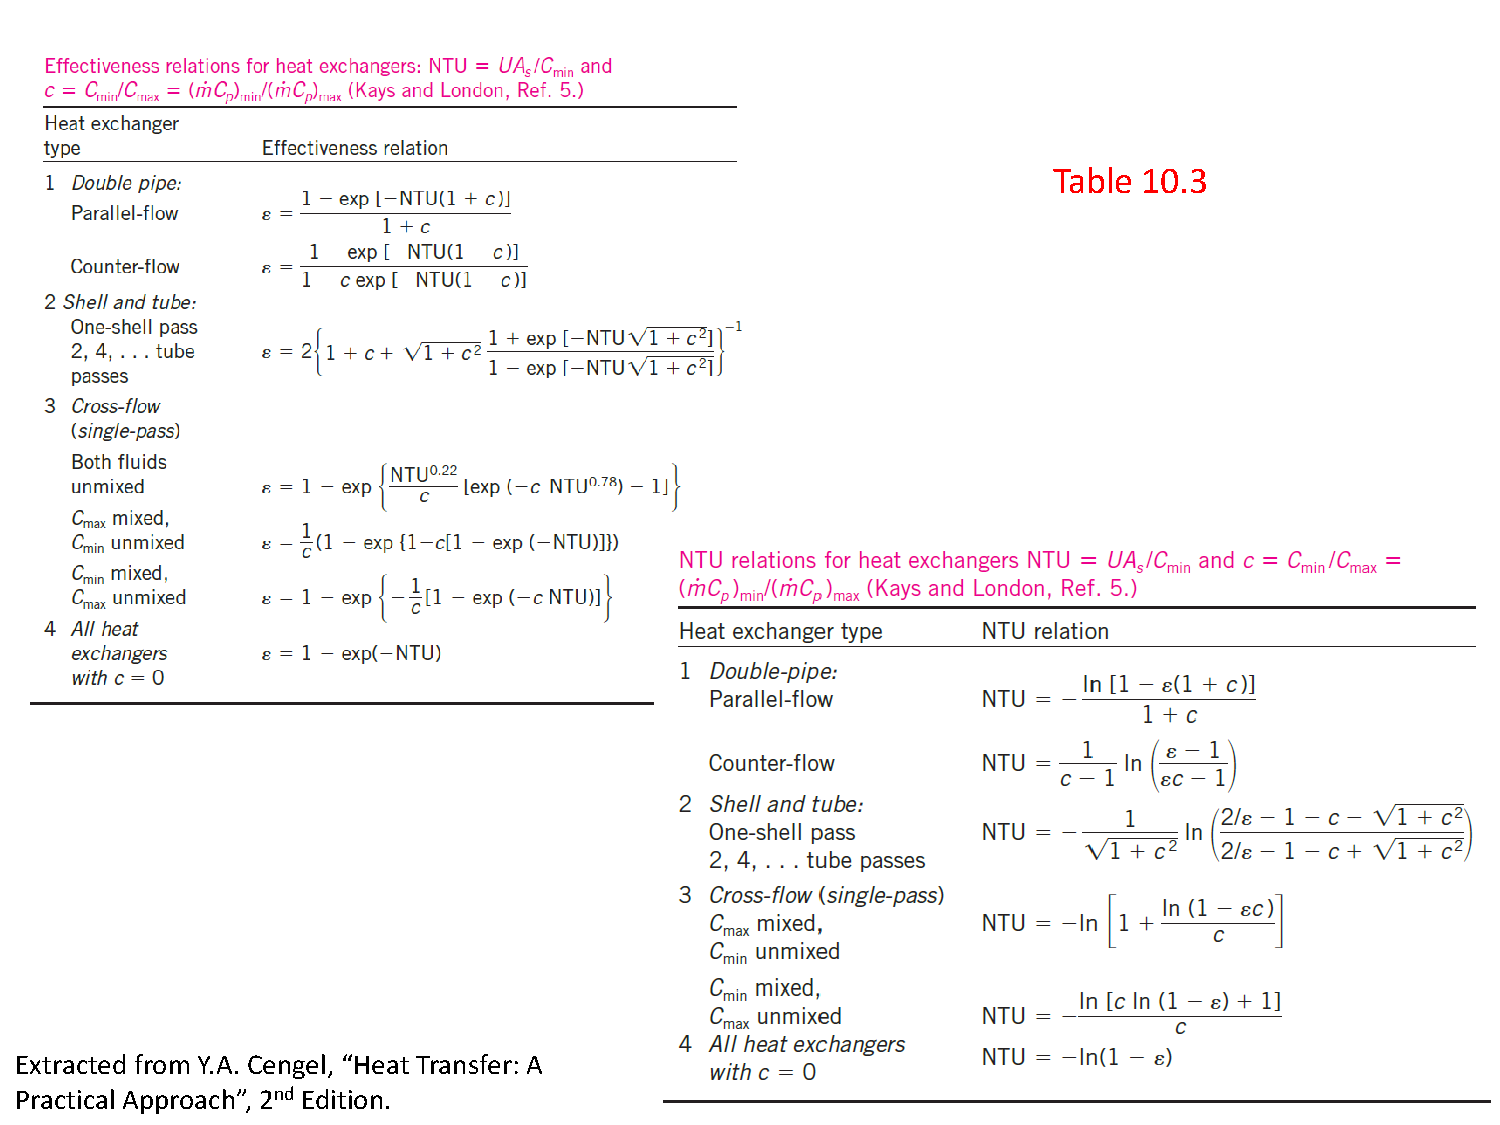
\includegraphics[width=1.\columnwidth,height=0.65\columnwidth,clip]{./Pics/HE_NTU1}
    \end{center}
\end{frame}
%%%
%%% Slide
%%%
\begin{frame}
  \frametitle{Appendix 2: Effectiveness-NTU Plots and Expressions}
    \begin{center}
         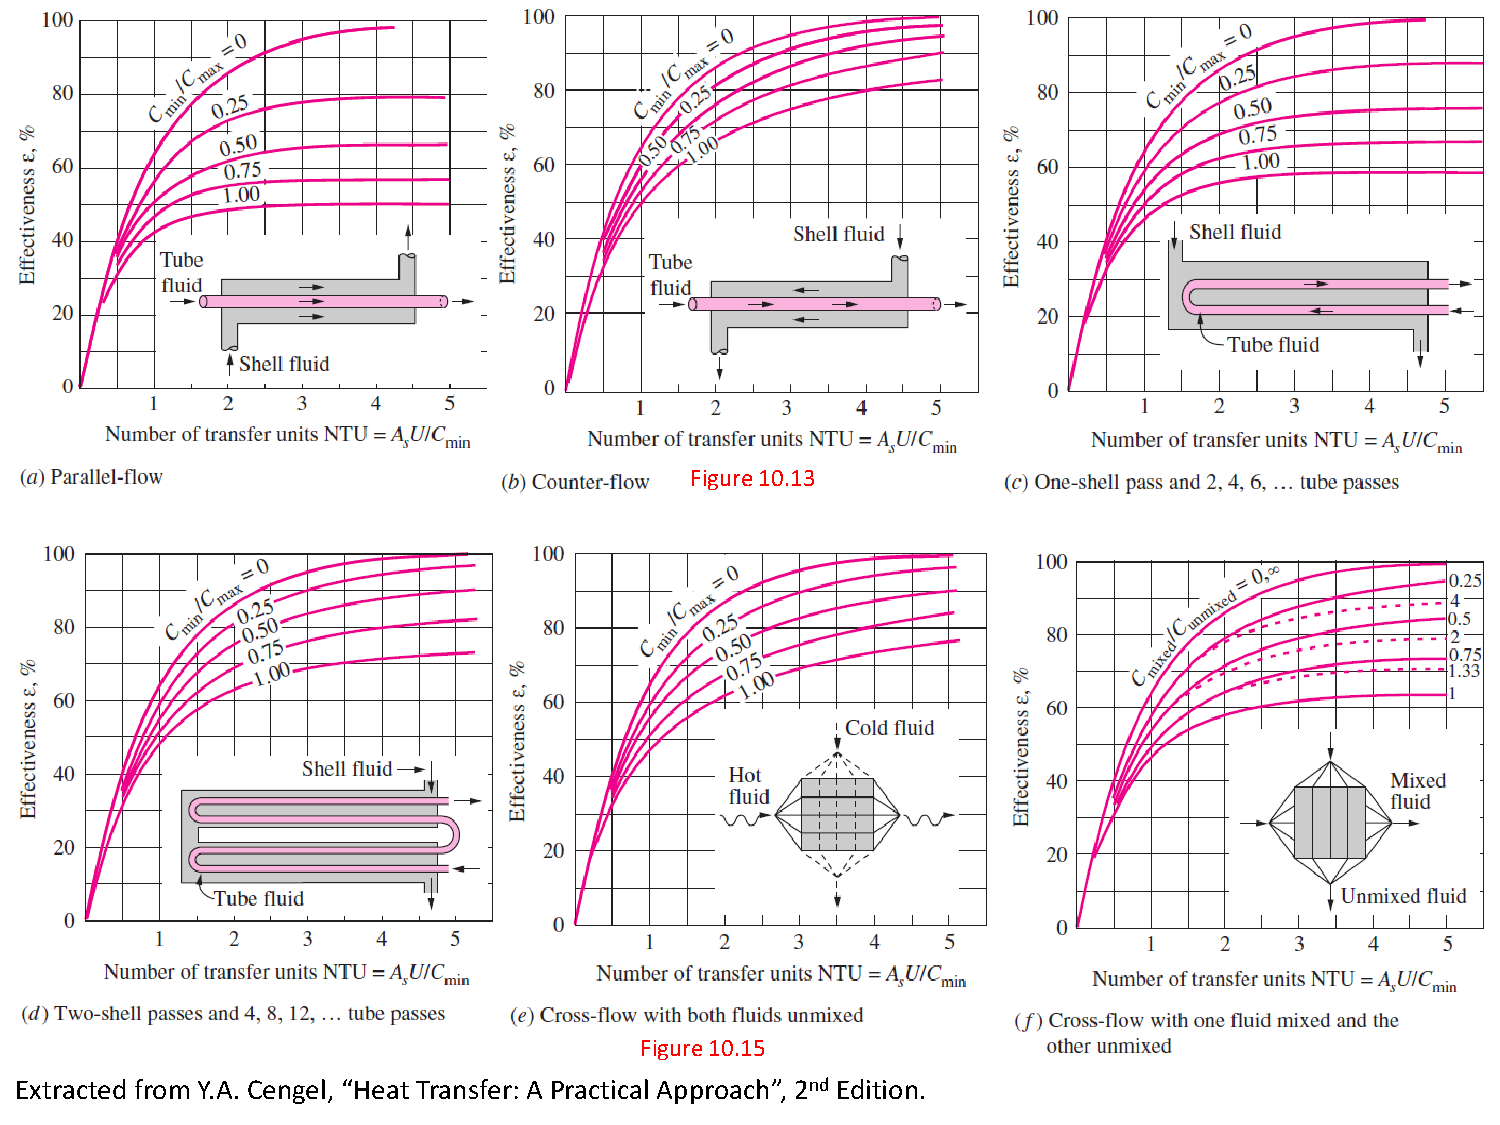
\includegraphics[width=1.\columnwidth,height=0.65\columnwidth,clip]{./Pics/HE_NTU2}
    \end{center}
\end{frame}


%{
%  \includepdf[pages=-,fitpaper]{./Pics/NTU.pdf}
%}

\end{document}
